\documentclass[twocolumn]{article}
\usepackage{amsmath}
\usepackage{xcolor}
\usepackage{graphicx}
\usepackage{caption}
\usepackage{fancyhdr}
\usepackage{geometry}
\usepackage{enumitem}
\usepackage{array}
\usepackage{hyperref}
\geometry{margin=0.7in}
\pagestyle{empty}

\begin{document}

\begin{figure}[t]
   % \begin{minipage}{0.45\linewidth}
        
\includegraphics[width=\linewidth]{img3.png} % Replace with actual image path
        %\end{minipage}\hfill
    %\begin{minipage}{0.45\linewidth}
        \textbf{Name: K.Saisusmitha} \\
        \textbf{Batch: 2} \\
        \textbf{ID: cometfwc018} \\
        \textbf{Date: 9th July 2025}
   % \end{minipage}
\end{figure}

\begin{center}
    {\LARGE \textbf{\textcolor{blue}{GATE Question Paper 2010, EC Question Number 39}}}
\end{center}

\vspace{1em}
\begin{figure}[h]
    \centering
    \includegraphics[width=\linewidth]{ec2010 39.png}
\caption*{\textbf{Figure: 4x1 MUX Circuit}}
\end{figure}

\section*{\textcolor{blue}{Question Analysis}}
\textbf{Given:} A 4x1 MUX circuit is shown with the inputs selected by variables $A$ and $B$ and data inputs driven by combinations of $C$ and $D$ logic. The Boolean function implemented by the circuit must be found.

\section*{Solution:}

\begin{enumerate}[label=\textbf{Step \arabic*:}]
    \item \textbf{Determine the Select Lines and MUX Inputs:} \\
    The 4x1 MUX uses $A$ and $B$ as the select lines:
    \[
    S_1 = A, \quad S_0 = B
    \]
    The MUX inputs are:
    \begin{align*}
        I_0 &= C \\
        I_1 &= D \\
        I_2 &= \overline{D} \\
        I_3 &= C \cdot \overline{D}
    \end{align*}

\item \textbf{Construct Output Expression:} \\
    Based on the select lines $(A,B)$, the output $F$ is:
    \[
    F(A,B,C,D) = 
    \begin{cases}
    I_0 = C & \text{if } A=0, B=0 \\
    I_1 = D & \text{if } A=0, B=1 \\
    I_2 = \overline{D} & \text{if } A=1, B=0 \\
    I_3 = C \cdot \overline{D} & \text{if } A=1, B=1
    \end{cases}
    \]
    Filling the truth table, the minterms where $F=1$ are: \\
    \[
    F = \sum m(0, 1, 3, 5, 9, 10, 14)
    \]
\end{enumerate}

\section*{\textcolor{blue}{Correct Option: (A)}}
\[
F = \sum m(0,1,3,5,9,10,14)
\]

\section*{\textcolor{blue}{Truth Table}}
\begin{table}[h]
\centering
\renewcommand{\arraystretch}{1.3}
\begin{tabular}{|c|c|c|c|c|}
\hline
A & B & Selected Input & Expression & Output (F) \\
\hline
0 & 0 & I0 = C & F = C & 1 if C=1 \\
0 & 1 & I1 = D & F = D & 1 if D=1 \\
1 & 0 & I2 = $\overline{D}$ & F = $\overline{D}$ & 1 if D=0 \\
1 & 1 & I3 = $C\cdot\overline{D}$ & F = $C\cdot\overline{D}$ & 1 if C=1, D=0 \\
\hline
\end{tabular}
\caption*{\textbf{Table: MUX Selection Logic}}
\end{table}

\section*{\textcolor{blue}{Hardware Implementation }}

\textbf{Logic Expression Inputs:} A, B, C, D — all controlled by push buttons.

\textbf{Output:} LED connected to GPIO pin shows value of F.

\subsection*{\textcolor{blue}{Hardware Requirements}}

\begin{table}[h]
\centering
\renewcommand{\arraystretch}{1.3}
\begin{tabular}{|c|l|}
\hline
\textbf{S.No} & \textbf{Component} \\ \hline
1 & Pico2W/Arduino \\
2 & Breadboard \\
3 & Push Buttons (4x) for Inputs A, B, C, D \\
4 & LED for Output F \\
5 & Resistors (220$\Omega$ for LED, 10k$\Omega$ for pull-downs) \\
6 & Jumper Wires \\
7 & Micro USB Cable \\
\hline
\end{tabular}
\caption*{\textbf{Table: Required Components}}
\end{table}

%\subsection*{\textcolor{blue}{GPIO Pin Connections}}

\begin{table}[h]
\centering
\renewcommand{\arraystretch}{1.3}
\begin{tabular}{|c|c|c|}
\hline
\textbf{Component} & \textbf{Pico2W Pin} & \textbf{Description} \\
\hline
Button A & GP14 & Select line S1 \\
Button B & GP15 & Select line S0 \\
Button C & GP16 & Input C \\
Button D & GP17 & Input D \\
LED (Output F) & GP13 & Output Logic \\
GND & GND & Common Ground \\
3.3V & 3.3V & Pull-up Supply \\
\hline
Button A & GP14 & Select line S1 \\
Button B & GP15 & Select line S0 \\
Button C & GP16 & Input C \\
Button D & GP17 & Input D \\
LED (Output F) & GP13 & Output Logic \\
GND & GND & Common Ground \\
3.3V & 3.3V & Pull-up Supply \\
\hline
\end{tabular}
\caption*{\textbf{Table: GPIO Pin Mapping}}
\end{table}

\subsection*{\textcolor{blue}{Steps to Upload Code using Pico2W}}

\begin{enumerate}
    \item Connect Pico 2 W via USB while holding BOOTSEL button.
    \item Drag-and-drop MicroPython file (only once).
    \item Open Thonny IDE and select MicroPython (Raspberry Pi Pico) as interpreter. If using a phone, use Micro REPL app.
    \item Write the MUX logic in Python using input reads and logical mapping.
    \item Connect the circuit as per table and test output LED for all input combinations.
\end{enumerate}
\section*{\textcolor{blue}{Arduino Uno Implementation}}

%\subsection*{\textcolor{blue}{GPIO Connections}}

\begin{table}%[H]
\centering
\renewcommand{\arraystretch}{1.3}
\begin{tabular}{|c|c|c|}
\hline
\textbf{Component} & \textbf{Arduino Pin} & \textbf{Description} \\
\hline
Button A & D2 & Select line S1 \\
Button B & D3 & Select line S0 \\
Button C & D4 & Input C \\
Button D & D5 & Input D \\
LED (Output F) & D6 & Output Logic \\
GND & GND & Common Ground \\
VCC & 5V & Pull-up Supply \\
\hline
\end{tabular}
\caption*{\textbf{Table: Arduino Pin Mapping}}
\end{table}

\subsection*{\textcolor{blue}{Steps to Upload Code to Arduino}}

\begin{enumerate}
    \item Connect Arduino Uno to PC using USB cable.
    \item Open Arduino IDE and select correct board and COM port.
    \item Write code for reading D2-D5 pins and generating logic for output F.
    \item Upload code using \textbf{Upload} button.
    \item Connect circuit as per connection table and validate using LED.
\end{enumerate}

%\section*{\textcolor{blue}{Truth Table (Verification)}}

\begin{table}[h]
\centering
\renewcommand{\arraystretch}{1.3}
\begin{tabular}{|c|c|c|c|c|c|c|}
\hline
A & B & C & D & Selected Input & Expression & F \\
\hline
0 & 0 & 0 & 0 & I0 & F = C             & 0 \\
0 & 0 & 0 & 1 & I0 & F = C             & 0 \\
0 & 0 & 1 & 0 & I0 & F = C             & 1 \\
0 & 0 & 1 & 1 & I0 & F = C             & 1 \\
0 & 1 & 0 & 0 & I1 & F = D             & 0 \\
0 & 1 & 0 & 1 & I1 & F = D             & 1 \\
0 & 1 & 1 & 0 & I1 & F = D             & 0 \\
0 & 1 & 1 & 1 & I1 & F = D             & 1 \\
1 & 0 & 0 & 0 & I2 & F = $\overline{D}$ & 1 \\
1 & 0 & 0 & 1 & I2 & F = $\overline{D}$ & 0 \\
1 & 0 & 1 & 0 & I2 & F = $\overline{D}$ & 1 \\
1 & 0 & 1 & 1 & I2 & F = $\overline{D}$ & 0 \\
1 & 1 & 0 & 0 & I3 & F = C$\cdot\overline{D}$ & 0 \\
1 & 1 & 0 & 1 & I3 & F = C$\cdot\overline{D}$ & 0 \\
1 & 1 & 1 & 0 & I3 & F = C$\cdot\overline{D}$ & 1 \\
1 & 1 & 1 & 1 & I3 & F = C$\cdot\overline{D}$ & 0 \\
\hline
\end{tabular}
\caption*{\textbf{Verification Table for MUX Logic}}
\end{table}
\section*{\textcolor{blue}{Conclusion}}
\begin{figure}
    \centering
    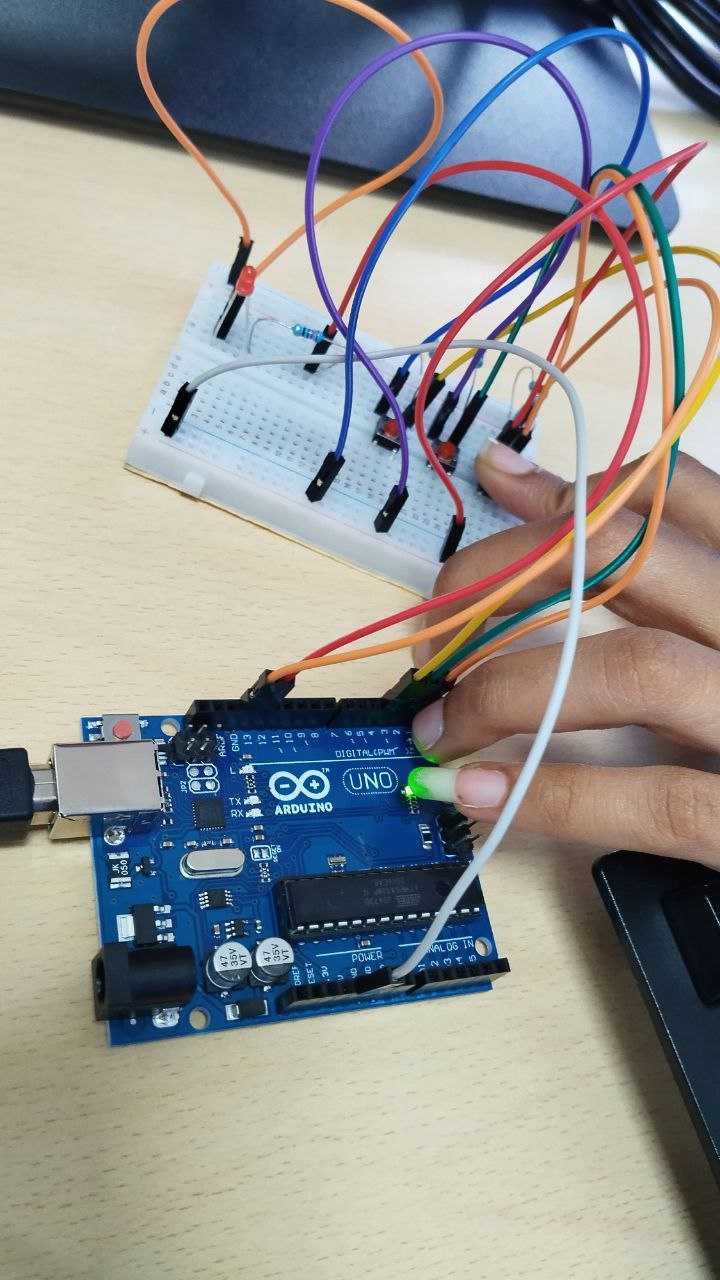
\includegraphics[width=0.95\linewidth]{ec39.jpg}
        \caption*{\textbf{Figure: Experiment using pico2w}}
\end{figure}
The logic function implemented using a 4x1 multiplexer was verified both theoretically and through a practical setup using Pico 2 W. Button inputs successfully mapped to select lines and MUX inputs, and the LED output validated the Boolean expression:
\[
F = \sum m(0,1,3,5,9,10,14)
\]

\section*{\textcolor{blue}{Source Code Link}}
The complete hardware simulation and code implementation for this experiment is available at the following GitHub repository:

\textbf{GitHub Repo:} \href{https://github.com/aisusmitha/FWC.git}{github.com/aisusmitha/FWC.git}
\end{document}
